\documentclass[aspectratio=169]{beamer}
\usepackage[utf8]{inputenc}
\usepackage{bookman}
\usetheme{Dresden}
\usepackage{graphicx}
\usepackage{hyperref}
\usepackage{todonotes}

\title[03-EDA-PCB]{EDA: PCB Layout}
\author{MedTech Prototyping Skills (BME290L)}
\institute[Palmeri (Spring 2023)]{Mark L. Palmeri, M.D., Ph.D.}
\date{February 09, 2023}
\logo{
\includegraphics[width=0.1\textwidth]{BME-HorizontalLogo-Web-Blue.png}}

\begin{document}

\frame{\titlepage}

\section{PCB}

\begin{frame}
  \frametitle{Why a PCB?}

  \begin{columns}
    \begin{column}{0.5\textwidth}
      \begin{itemize}
        \item Breadboards are good for simple testing, but not robust.
        \item Need to reduce form factor.
        \item Reduce noise, capacitive effects, etc.
        \item SMD (versus thru-hole) components are becoming ubiquitous.
      \end{itemize}
    \end{column}
    \begin{column}{0.5\textwidth}
      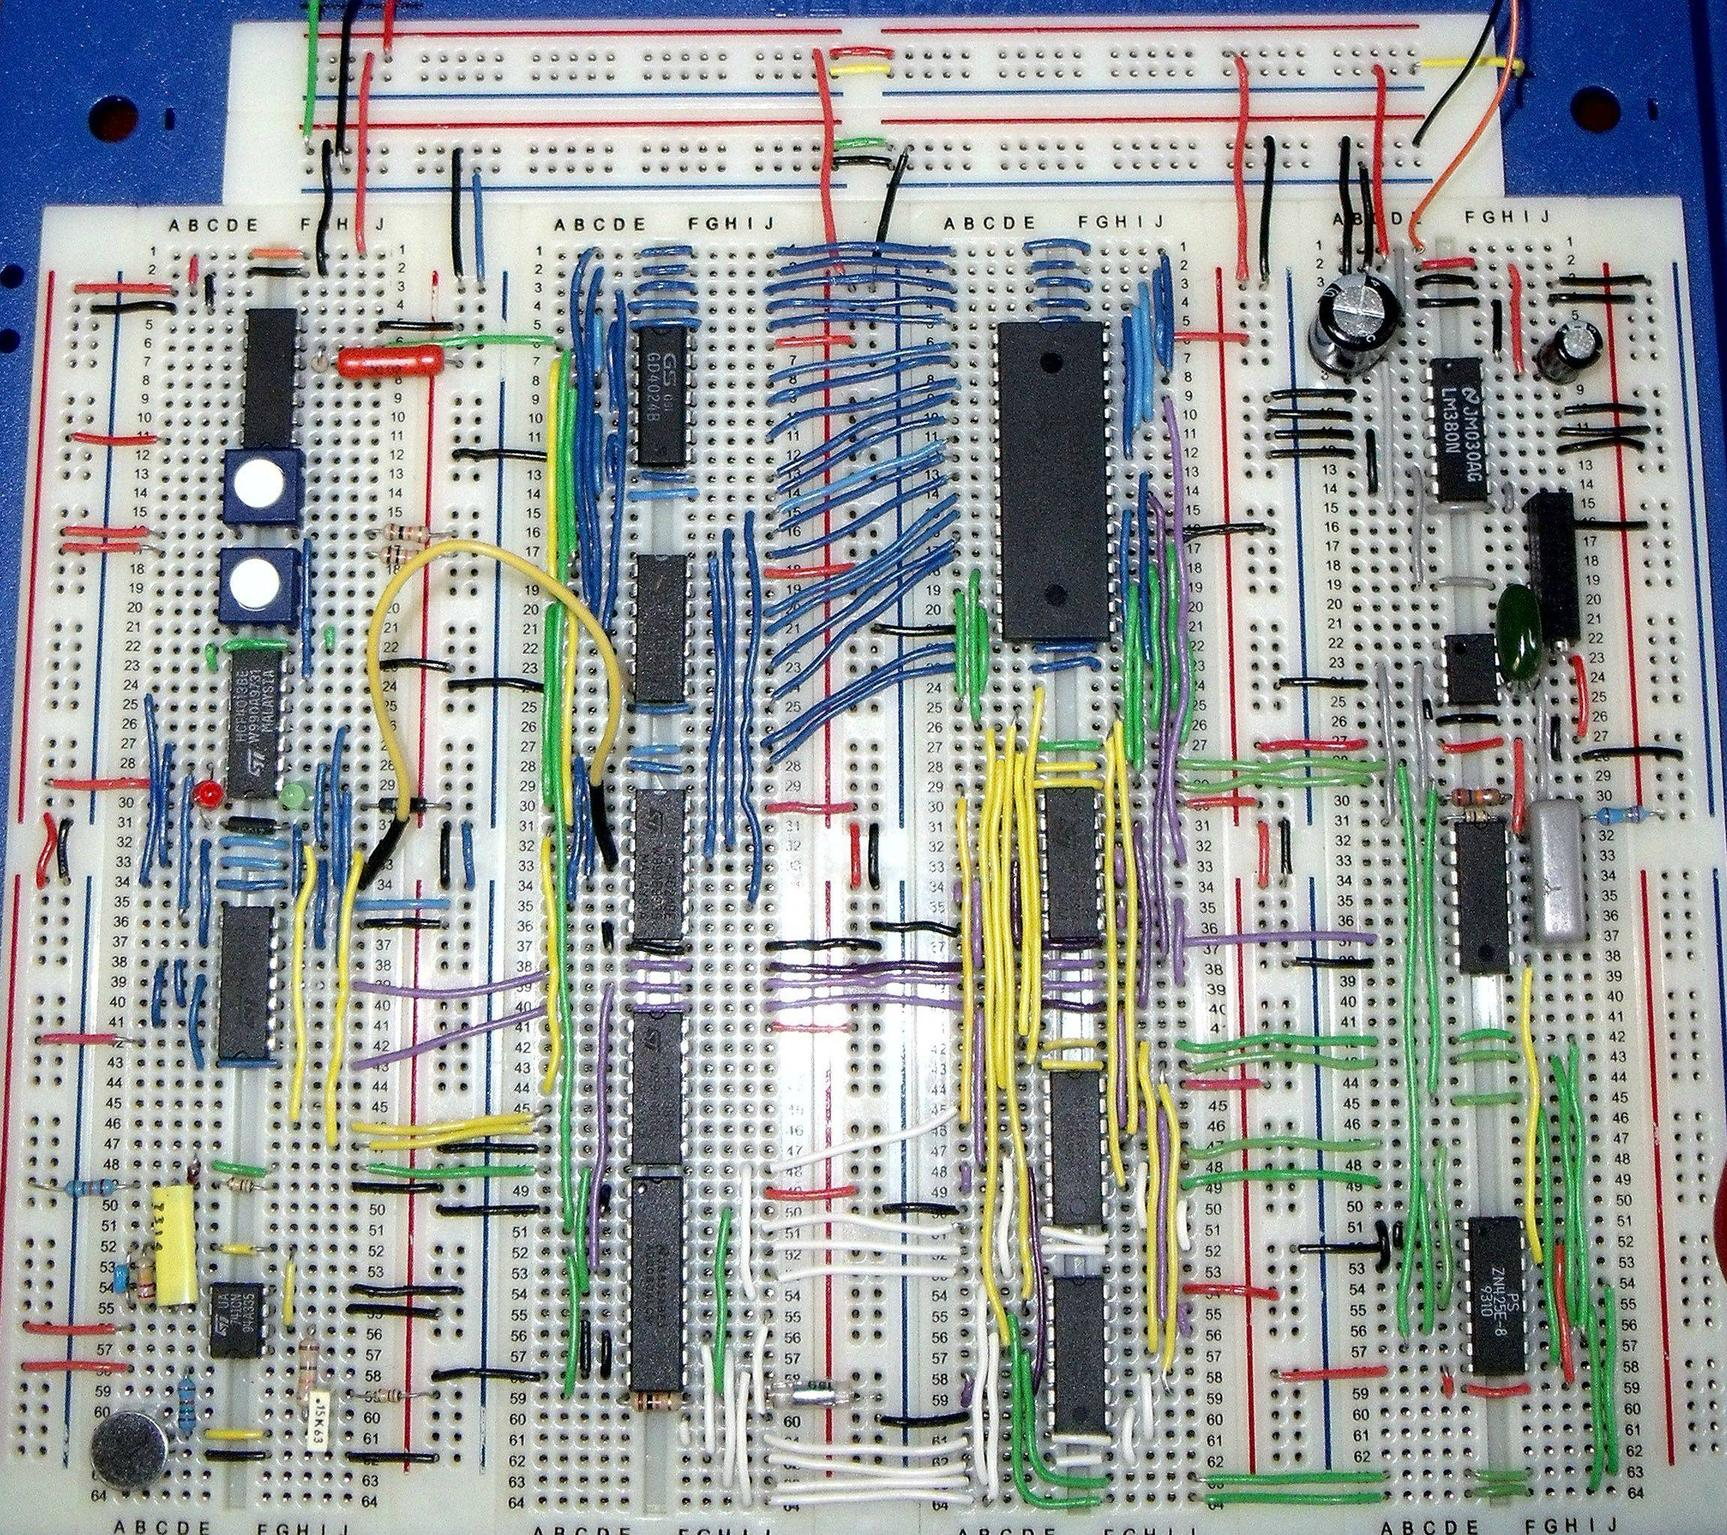
\includegraphics[width=1.0\textwidth]{breadboard.jpg} 
    \end{column}
  \end{columns}
\end{frame}

\begin{frame}
  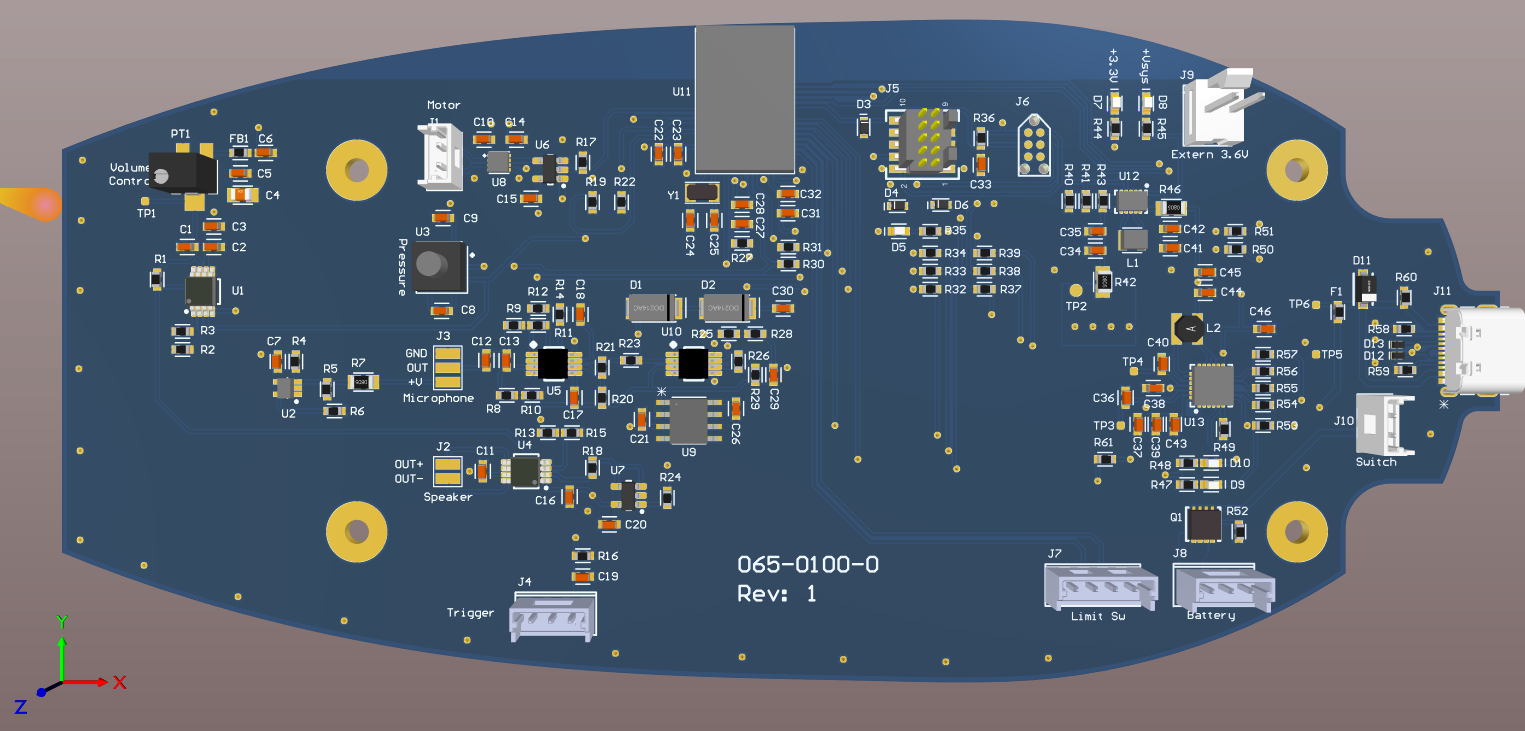
\includegraphics[width=1.0\textwidth]{pcb_rev1.png}
\end{frame}

\begin{frame}
  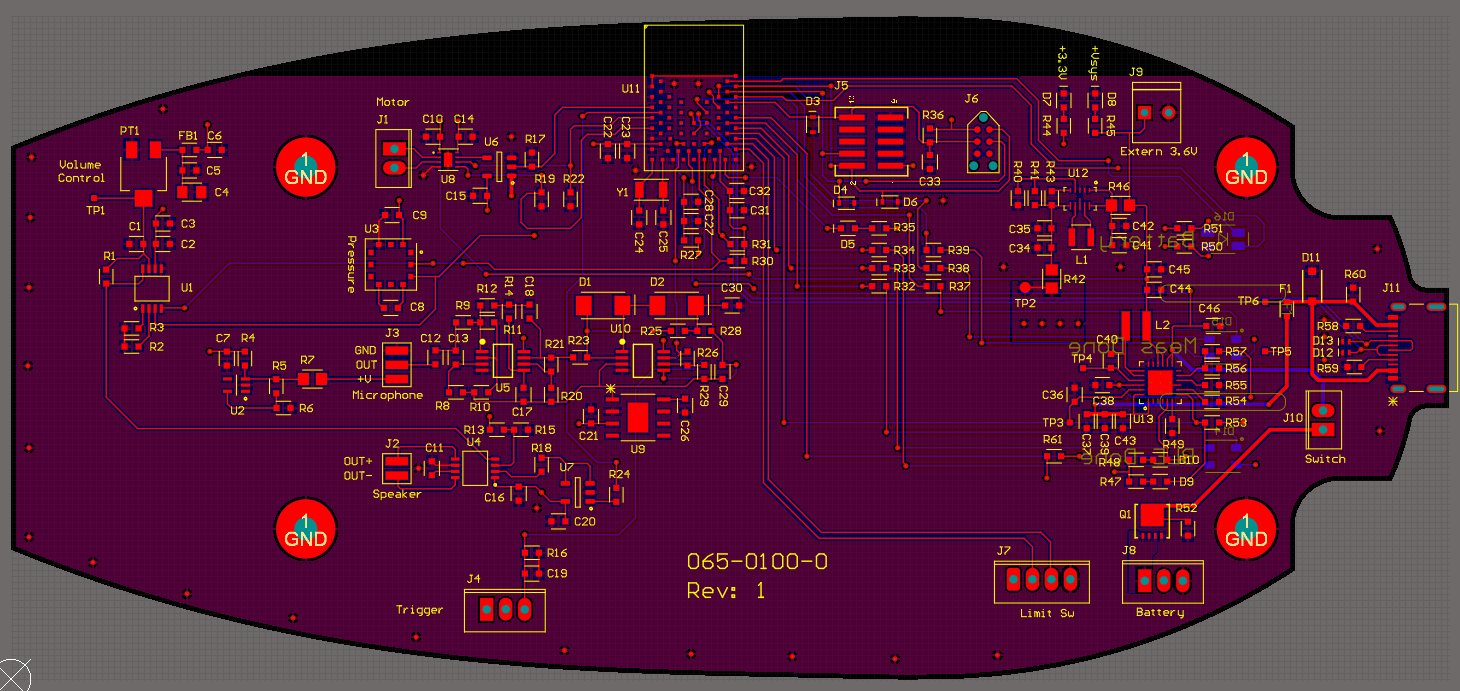
\includegraphics[width=1.0\textwidth]{pcb_layout_rev1.png}
\end{frame}

\begin{frame}
  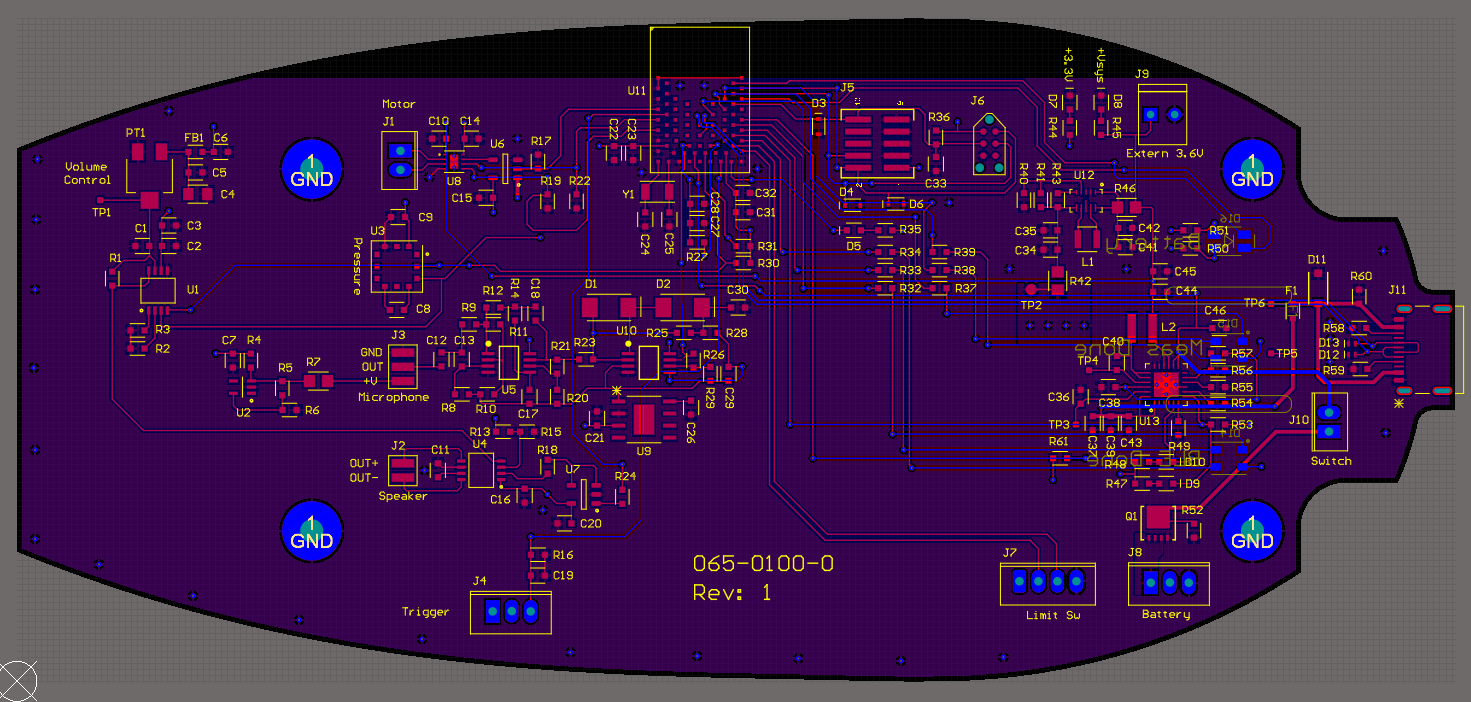
\includegraphics[width=1.0\textwidth]{pcb_layout_rev1_bottom.png}
\end{frame}

\begin{frame}
  \frametitle{Two-layer PCB}

  \begin{columns}
    \begin{column}{0.5\textwidth}
      \begin{itemize}
        \item Single-layer boards for ``trivial'' layouts.
        \item Two-layer board best balance of flexibility and complexity for ``simple'' layouts.
        \item $>$ 2 layers increases complexity (but putting power and ground on
        their own layers can be advantageous)
      \end{itemize}  
    \end{column}
    \begin{column}{0.5\textwidth}
      \centerline{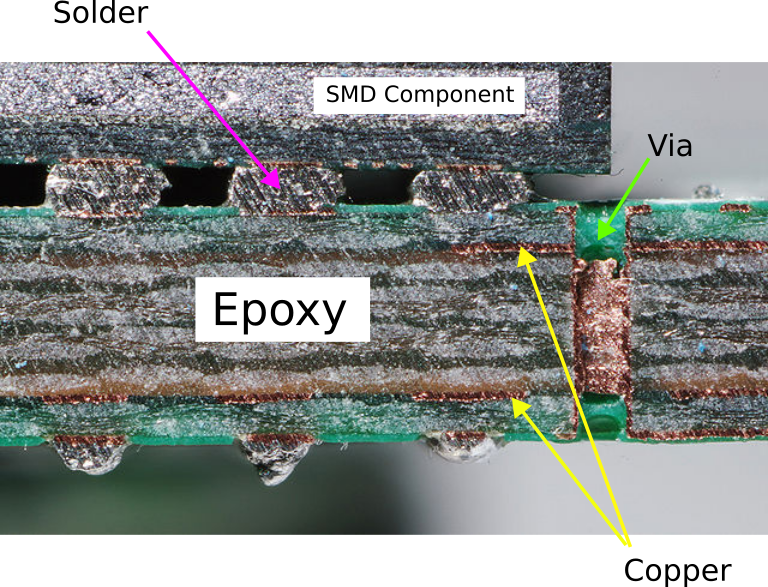
\includegraphics[width=1.0\textwidth]{pcb_layers_annotated.png}}
    \end{column}
  \end{columns}

\end{frame}

\begin{frame}
  \frametitle{THT vs. SMD}
  \begin{columns}
    \begin{column}{0.5\textwidth}
      \begin{itemize}
        \item Surface mount components on the same side as the traces
        \item Soldering using reflow.
        \item Thru-hole components on the opposite side from the traces (ease of
        soldering).
      \end{itemize}
    \end{column}
    \begin{column}{0.5\textwidth}
      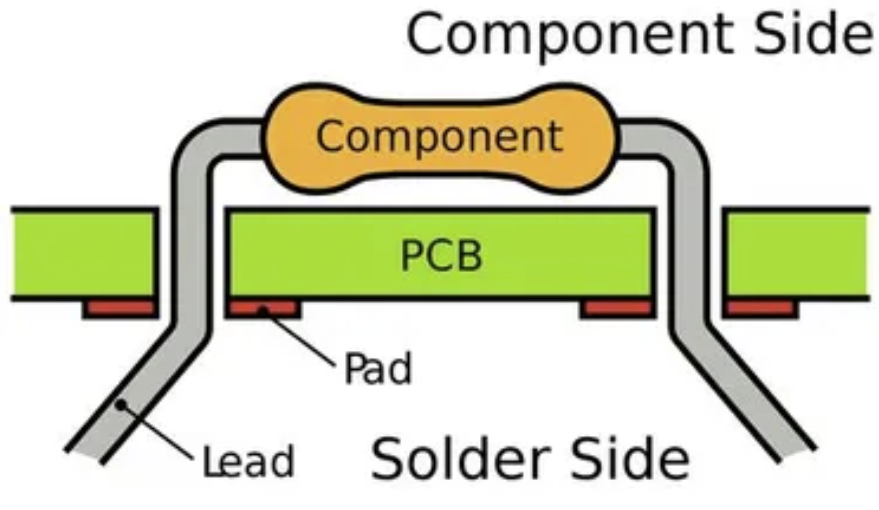
\includegraphics[width=0.75\textwidth]{tht_component.png}\\
      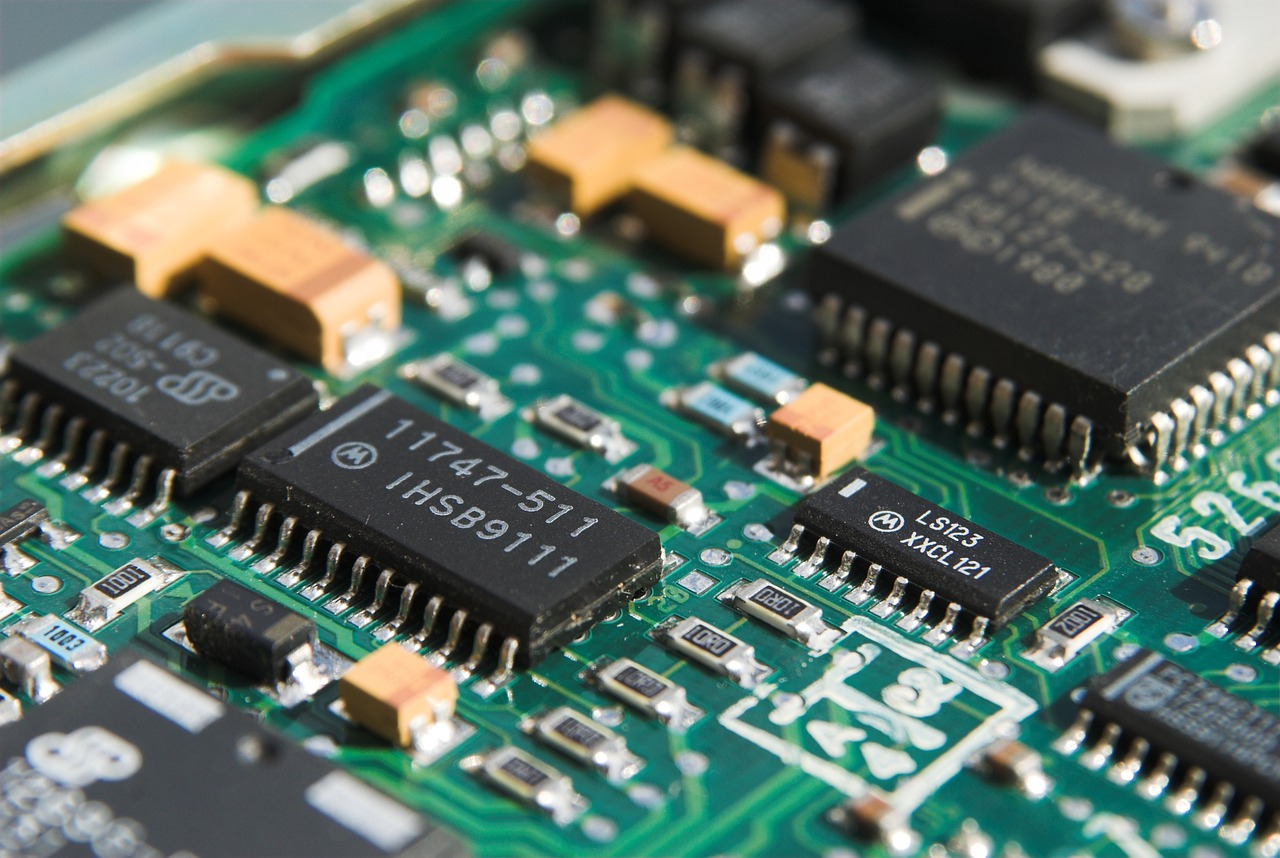
\includegraphics[width=0.65\textwidth]{smd_components.jpg}
    \end{column}
  \end{columns}
\end{frame}

\section{Workflow}

\begin{frame}
  \frametitle{PCB Editor}
  \centerline{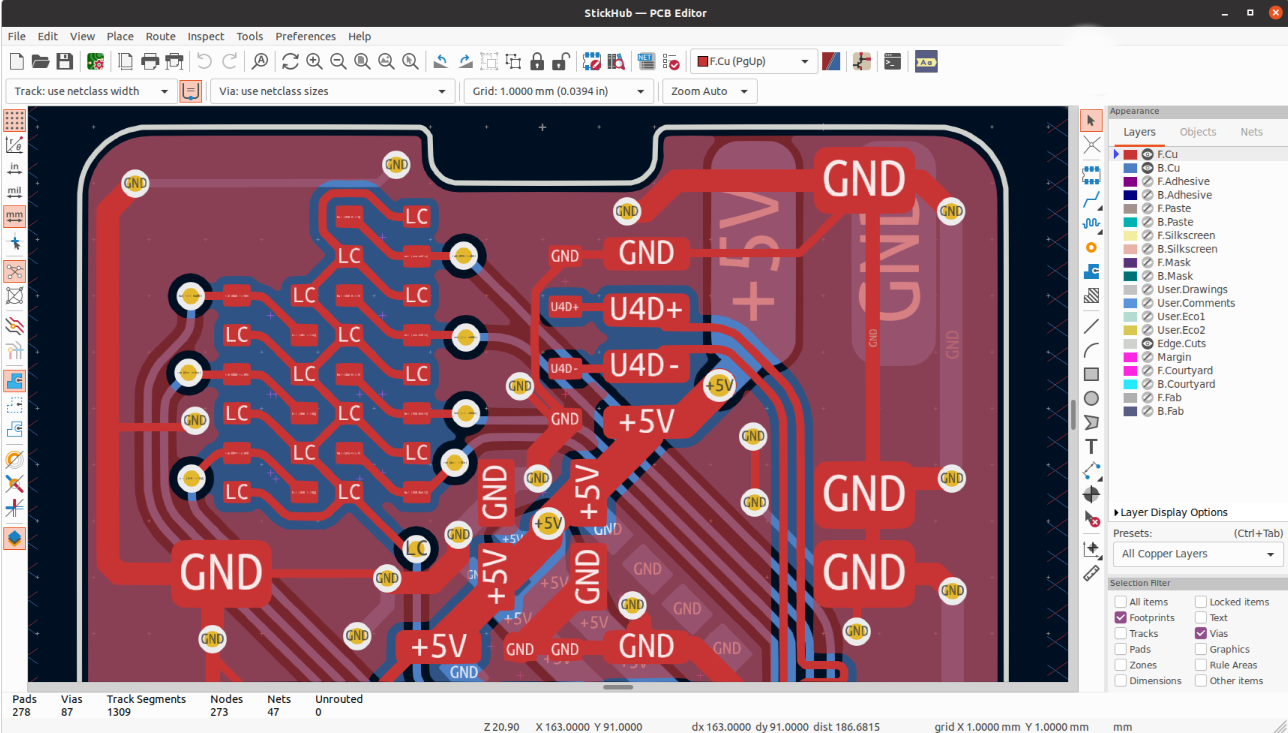
\includegraphics[width=0.8\textwidth]{pcbnew_ui.png}}
\end{frame}

\frame{
  \frametitle{Laying out a PCB}
  \begin{enumerate}
    \item Make sure that all parts are \textbf{annotated} and have \textbf{footprints}.
    \item Create PCB from schematic
    \item All component pins/pads that need to be connected with traces will be connected with airwires.
    \item Use \texttt{Graphics Lines} tool to create board outline (Layer:
    \texttt{Edge.Cuts})
    \item Layout components based on your design needs / constraints,
    considering orientation, board side, etc.
    \item Setup \textbf{Design Rules} (\texttt{File $\rightarrow$ Board Setup...}):
    \begin{itemize}
        \item Trace width ($\geq$ 20 mil)
        \item Drill diameter ($\geq$ 1 mm)
        \item Clearance ($\geq$ 32 mil)
    \end{itemize}
    \item Setup \textbf{Net Classes} for signal and power/ground (wider / more clearance).
  \end{enumerate}
}

\begin{frame}
  \frametitle{Laying out a PCB}
  \begin{enumerate}
    \setcounter{enumi}{7}
    \item Route traces
    \begin{itemize}
      \item Make sure that you are on the correct layer! 
    \end{itemize}
    \item Use \texttt{Filled Zone} tool to create a copper pour
    (\texttt{F/B.Cu}), usually associated with the \texttt{GND} net.
    \item Clearout other zones, as needed.
    \item Perform \textbf{Design Rule Check (DRC)}
  \end{enumerate}
\end{frame}


\section{Power / Ground}

\begin{frame}
  \frametitle{Power Traces / Layers}

  \begin{columns}
    \begin{column}{0.5\textwidth}
      \begin{itemize}
        \item Larger trace width for greater power delivery (less resistance for
        more current).
        \item Even better to dedicate an entire layer
        \begin{itemize}
          \item More direct return paths
          \item Shielding (EMI)
          \item Reduce noise (switching)
          \item Dissipate heat
        \end{itemize}
      \end{itemize}
    \end{column}
      \begin{column}{0.5\textwidth}
        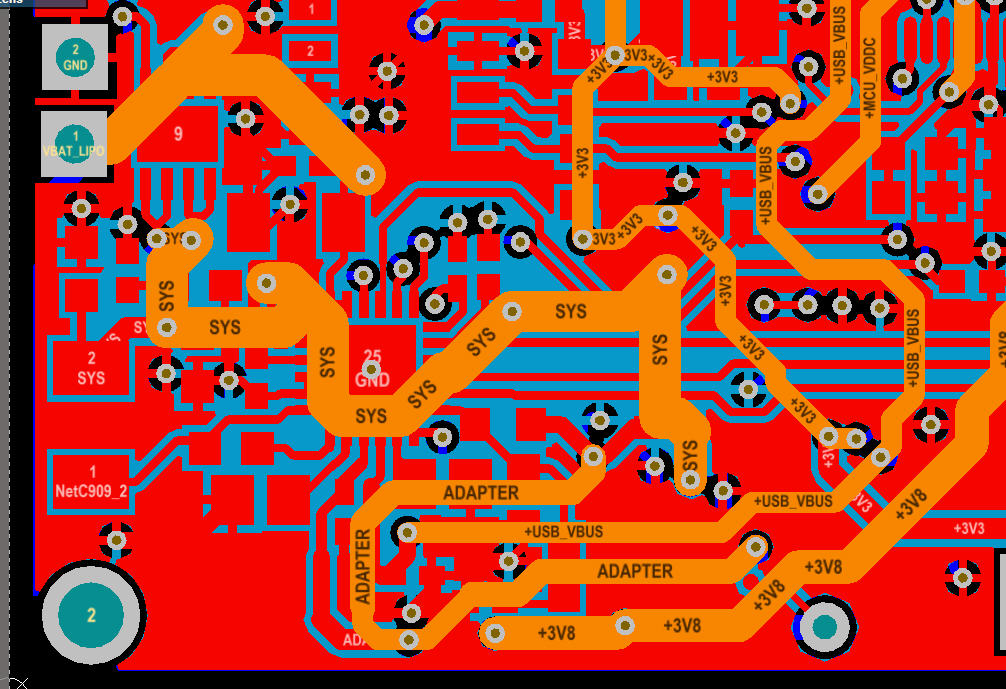
\includegraphics[width=1.0\textwidth]{pwr_vs_signal_traces.jpg}
      \end{column}
  \end{columns}

\end{frame}

\frame{
  \frametitle{Copper Ground Pours}
  \begin{columns}
    \begin{column}{0.5\textwidth}
    \begin{itemize}
      \item Help reject noise \& interference
      \item Lower impedance to ground
      \item Save milling time and bits!!
      \item Use jumper wire connections to electrically connect \texttt{GND} ``islands''.
    \end{itemize}
    \end{column}
      \begin{column}{0.5\textwidth}
        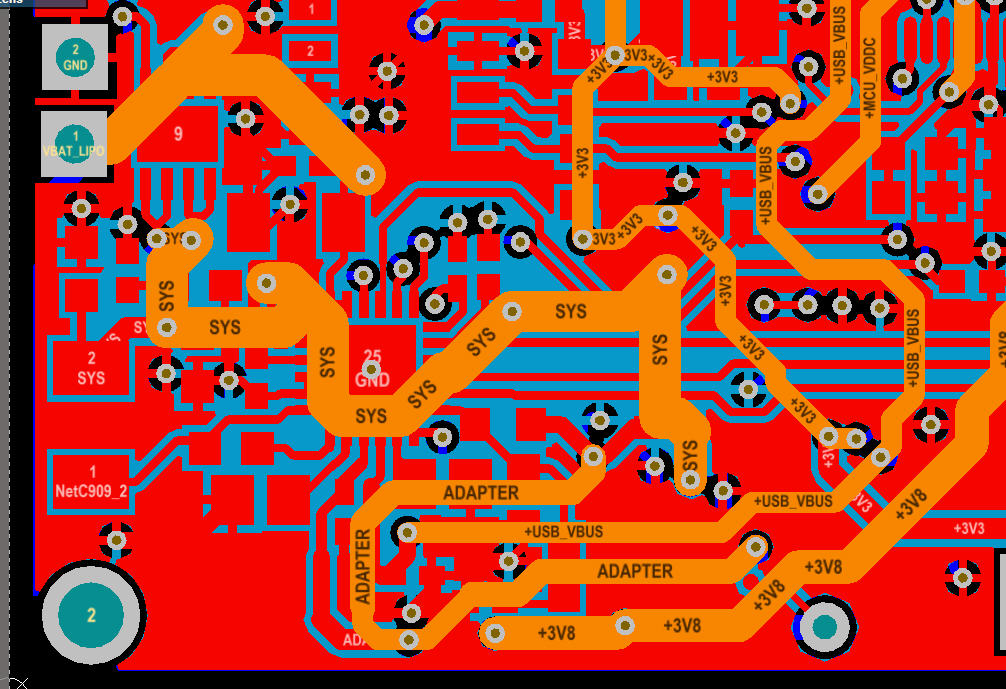
\includegraphics[width=1.0\textwidth]{pwr_vs_signal_traces.jpg}
      \end{column}
  \end{columns}
}

\begin{frame}
  \frametitle{Reducing Noise}
  \begin{itemize}
    \item Separate analog (\texttt{AGND}) and digital grounds (\texttt{GND}),
    and electrically connect using a \textbf{Net Tie}.
    \item Reduce trace ``loops'' (RF interference)
    \item Place decoupling capacitors next to power pins they are supporting.
  \end{itemize}
\end{frame}

\begin{frame}
    \frametitle{Thermal Relief}

    \centerline{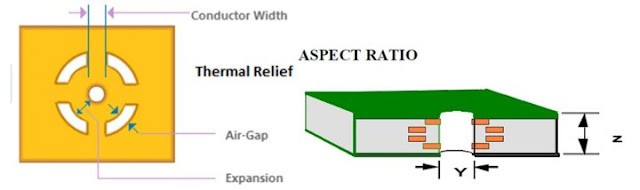
\includegraphics[width=0.75\textwidth]{thermal_relief.jpg}}

\end{frame}


\section{Tips}

\frame{
  \frametitle{Kinds of Grounds}

  \begin{columns}
  \begin{column}{0.5\textwidth}
    \centerline{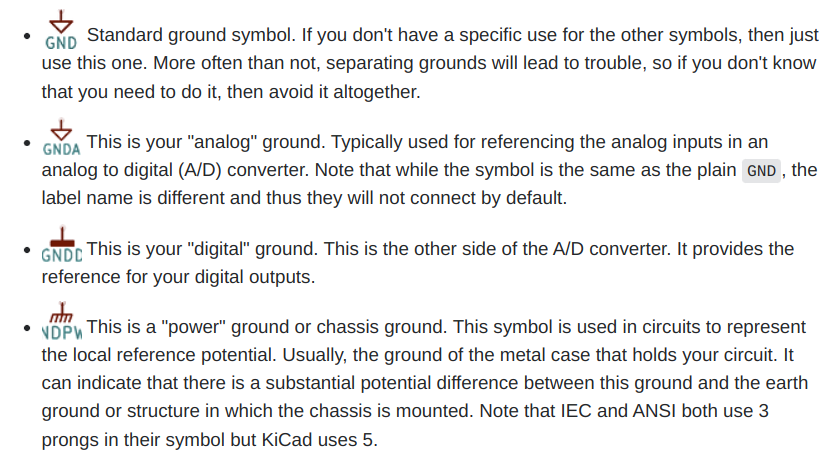
\includegraphics[width=1.0\textwidth]{grounds01.png}}
  \end{column}
  \begin{column}{0.5\textwidth}
    \centerline{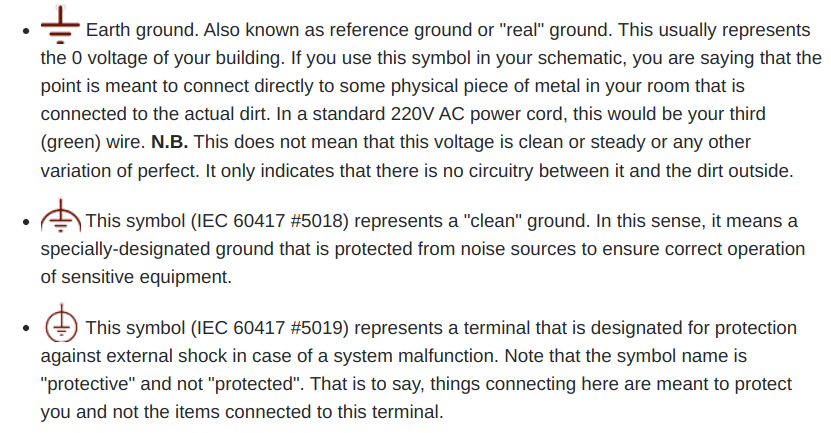
\includegraphics[width=1.0\textwidth]{grounds02.png}}
  \end{column}
\end{columns}

\begin{tiny}
\url{https://electronics.stackexchange.com/questions/392911/kicad-5-what-is-the-significance-of-the-various-gnd-symbols}
\end{tiny}
}

\frame{
  \frametitle{Tips-n-Tricks}
  \begin{itemize}
      \item You need to make sure that you update your PCB everytime you edit
      your schematic.  Failing to do so will create asyncrony of the two
      documents, which will be \emph{painful} to resolve.
     \item Clean up airwires with the \texttt{Ratsnest} tool.
     \item \textbf{Vias}: connections between top and bottom layers of a board.
     These can be plated or connected with a physical wire.
     \item Use jumpers for wire connections.
     \item Strategically place test pins / pads.
     \item Define ``clearout'' zones for areas where components cannot be placed
     (e.g., RF antenna)
     \item $\pm$ connections can be routed as a \textbf{Differential Pair}.
    \end{itemize}
}

\begin{frame}
  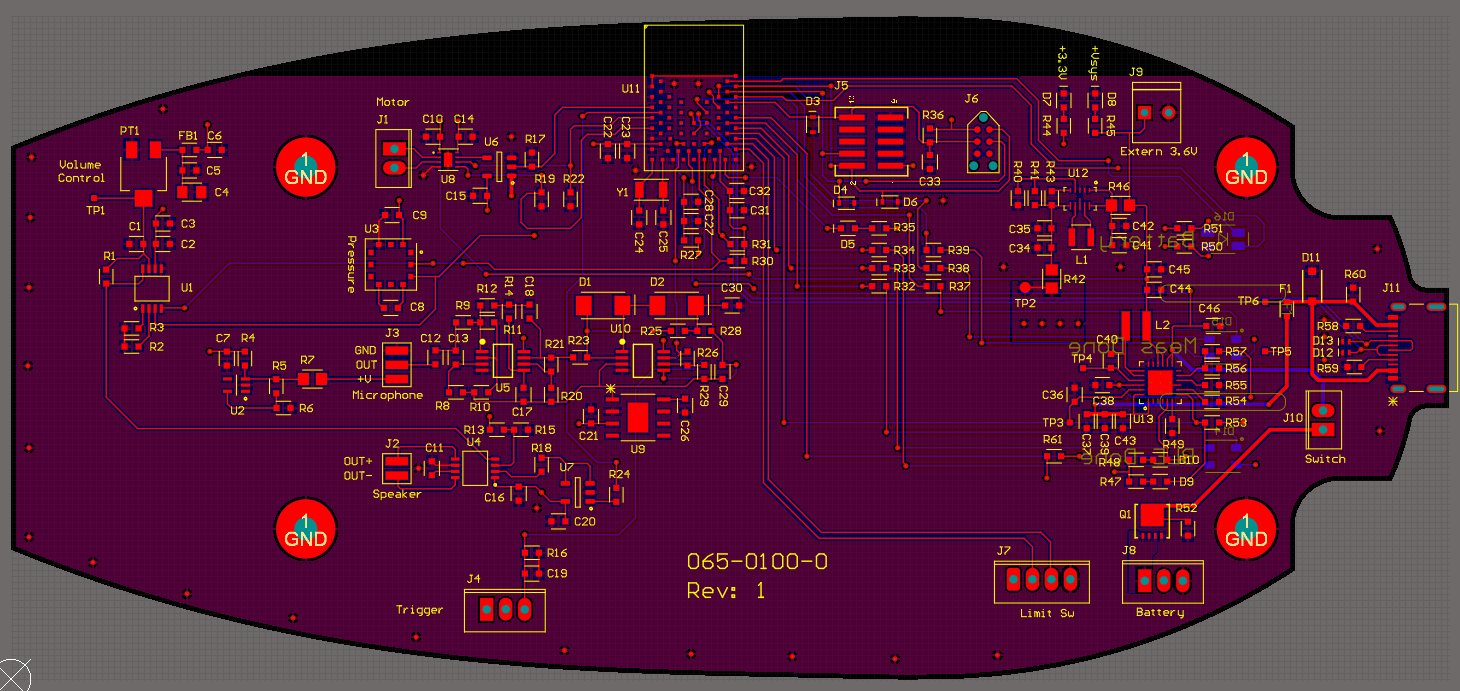
\includegraphics[width=1.0\textwidth]{pcb_layout_rev1.png}
\end{frame}

\begin{frame}
  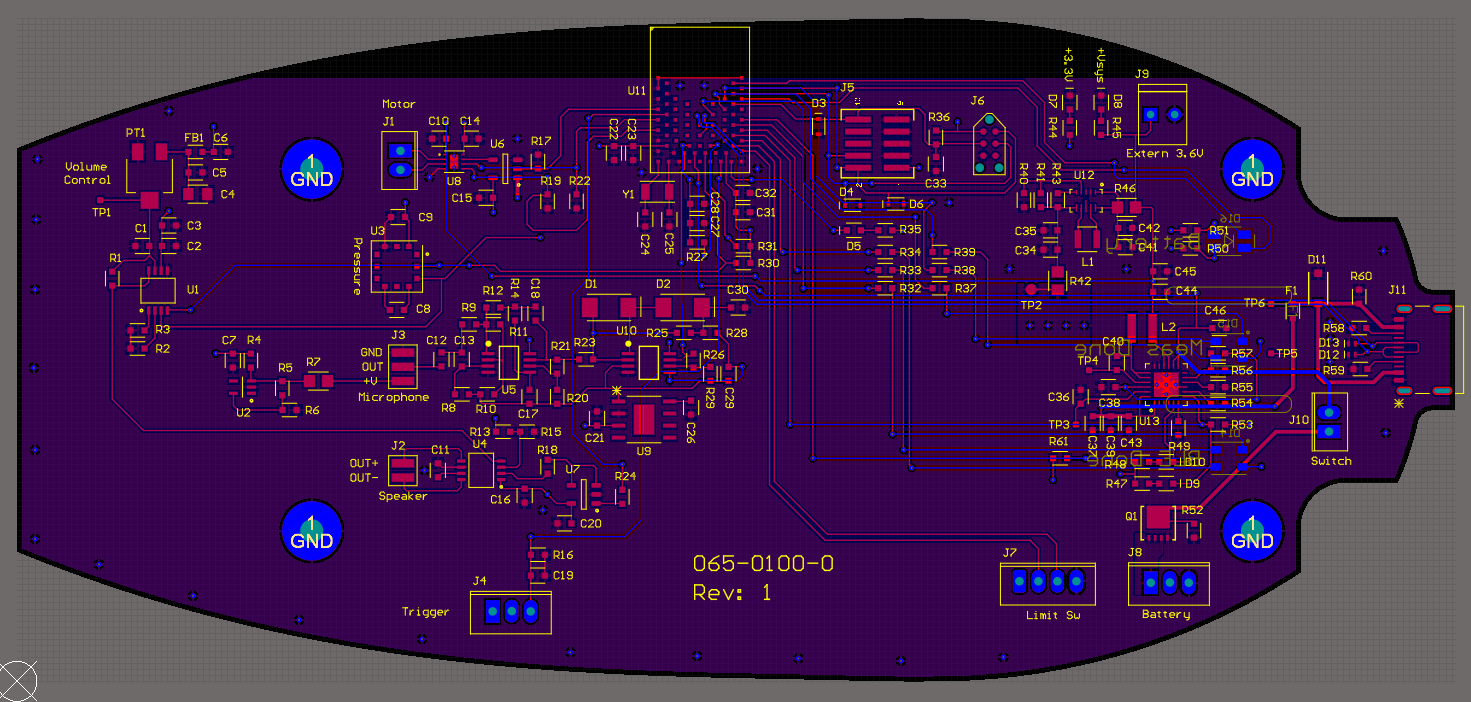
\includegraphics[width=1.0\textwidth]{pcb_layout_rev1_bottom.png}
\end{frame}

\begin{frame}
  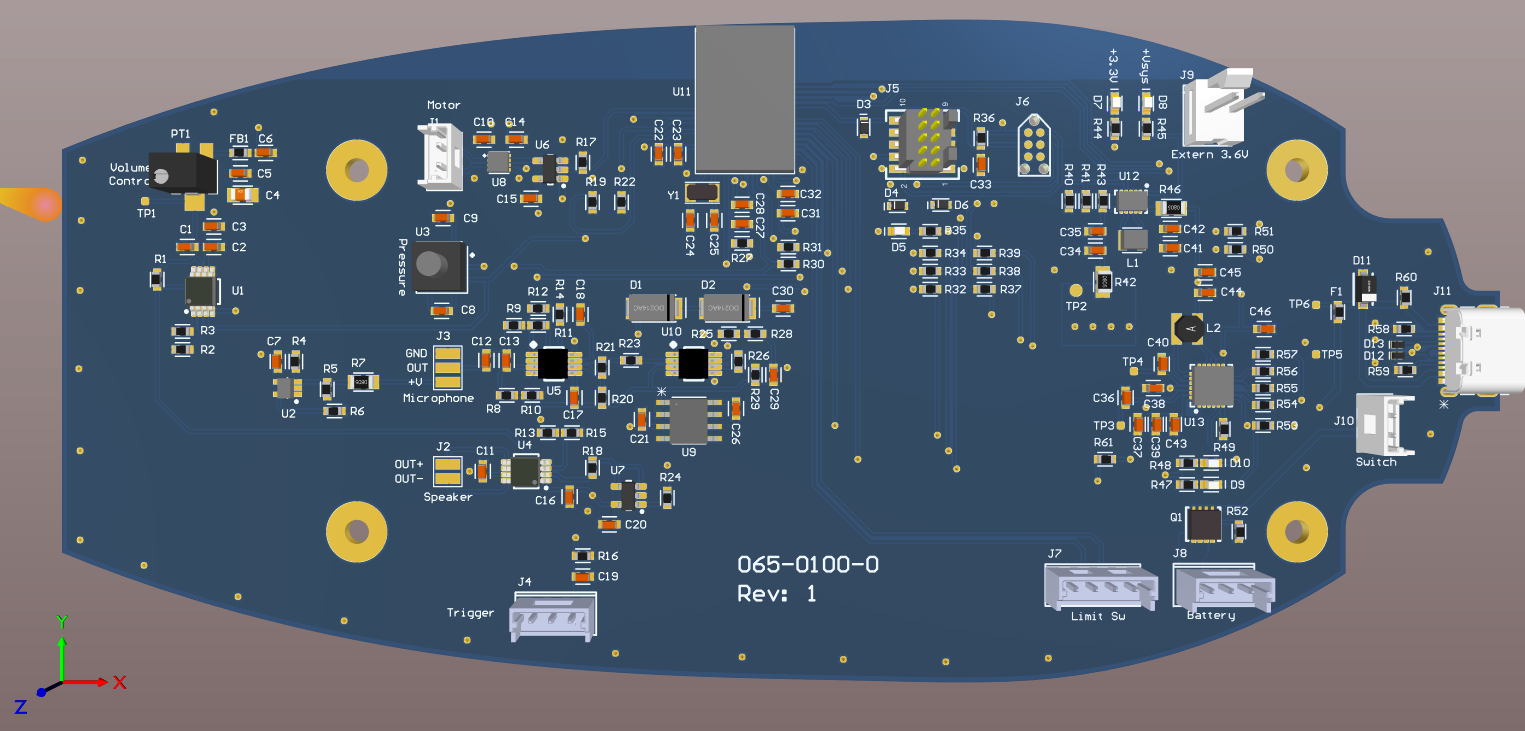
\includegraphics[width=1.0\textwidth]{pcb_rev1.png}
\end{frame}

\section{Resources}

\begin{frame}
  \frametitle{Resources}
  \begin{itemize}
    \item \href{https://learn.sparkfun.com/tutorials/pcb-basics}{PCB Basics (SparkFun)}
    \item \href{https://mlp6.pages.oit.duke.edu/Medical-Electrical-Equipment/How\_to\_Design\_the\_Perfect\_PCB.pdf}{How to Design the Perfect PCB}
    \item \href{https://docs.kicad.org/6.0/en/pcbnew/pcbnew.html}{KiCad Docs: PCB Editor}
    \item \href{https://gitlab.oit.duke.edu/mlp6/kicad_test}{Example KiCad Project}
    \item \href{https://resources.pcb.cadence.com/blog/2020-grounding-and-voltage-routing-considerations-in-pcb-design-e2ek}{Grounding and Voltage Routing Considerations in PCB Design}
    \item \href{https://resources.pcb.cadence.com/blog/2021-effective-pcb-trace-width-and-spacing}{Effective PCB Trace Width and Spacing}
  \end{itemize}
\end{frame}

\end{document}
